\documentclass[11pt]{article}
\usepackage[margin=0.88in]{geometry}
\usepackage{amsmath,amssymb,amsthm}
\usepackage[T1]{fontenc}
\usepackage{lmodern}
\usepackage{graphicx}
\usepackage[hidelinks]{hyperref}
\usepackage{xcolor}

\newtheorem{theorem}{Theorem}
\newtheorem{corollary}[theorem]{Corollary}
\newtheorem{remark}[theorem]{Remark}
\newcommand{\N}{\mathbb N}
\newcommand{\D}{\mathcal D}

\title{A Finite-Gap Reduction for the Haar-Liminf Problem}
\author{Candidate partial result for arXiv:2603.17983 and arXiv:2212.11229}
\date{12 August 2026}

\begin{document}
\maketitle

\begin{center}
\fcolorbox{black}{gray!8}{\parbox{0.91\linewidth}{
\textbf{Status: candidate partial result, likely valid.}
For a symmetric polynomial hypergroup, if the $n$th Haar weight satisfies
$h(n)<2$, then the Hermitian dual has at least $n$ gaps inside the convex
hull of the orthogonalization measure.  Hence every polynomial hypergroup
whose dual has only finitely many such gaps satisfies $h(n)\geq2$ eventually,
and therefore $\liminf h(n)\geq2$.  The unrestricted infinite-gap case is
not settled.}}
\end{center}

\section{The residual open problem}

Let $(P_n)_{n\geq0}$ be a symmetric random-walk polynomial sequence,
normalized by $P_n(1)=1$, and suppose that products have nonnegative
linearization
\begin{equation}\label{eq:lin}
 P_mP_n=\sum_{k=|m-n|}^{m+n}g(m,n;k)P_k,
 \qquad g(m,n;k)\geq0,
 \qquad \sum_k g(m,n;k)=1.
\end{equation}
Let $\mu$ be its orthogonalization probability measure and let
\begin{equation}\label{eq:haar}
 h(n)=\frac{1}{\int P_n(x)^2\,d\mu(x)}
     =\frac{1}{g(n,n;0)}
\end{equation}
be the Haar weight.  Kahler and Szwarc asked whether every such polynomial
hypergroup satisfies
\[
 \liminf_{n\to\infty}h(n)\geq2.
\]
Their exact list of open problems is reproduced below.

\begin{figure}[ht]
  \centering
  
\includegraphics[width=0.97\textwidth]{figures/open_problem_crop.png}
  \caption{The residual Haar-liminf question in Kahler--Szwarc,
  arXiv:2212.11229v3, PDF page 24 (the page is numbered 24 in the text).}
\end{figure}

The later paper arXiv:2603.17983 constructs examples with $h(2)<2$ and
thereby fully answers the older pointwise Questions (i) and (iii).  It says
that its construction gives only partial answers to Questions (iv) and (v),
whose asymptotic clauses contain the same liminf issue.

\begin{figure}[ht]
  \centering
  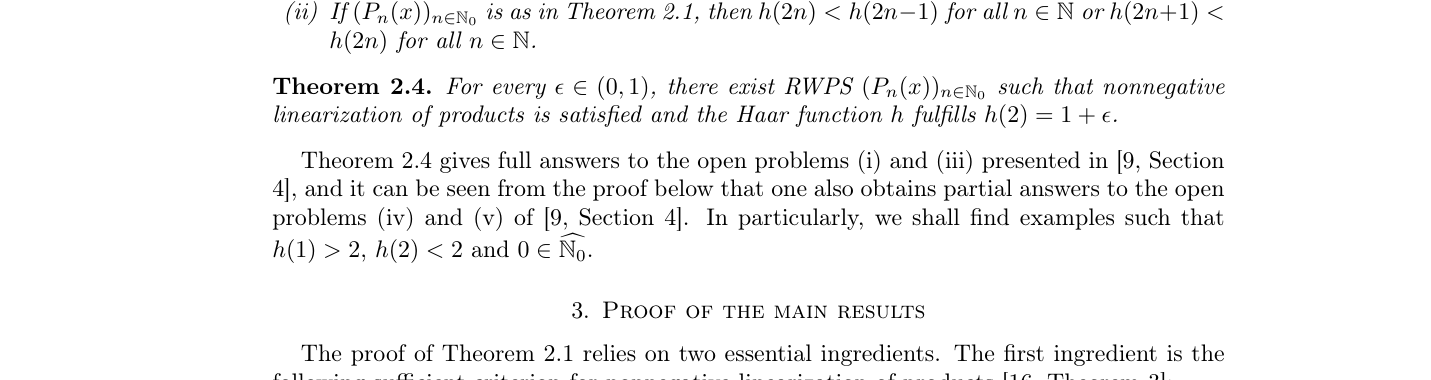
\includegraphics[width=0.97\textwidth]{figures/current_partial_crop.png}
  \caption{Theorem 2.4 and the authors' scope statement in
  arXiv:2603.17983, PDF page 6.}
\end{figure}

\section{The gap obstruction}

Write
\[
 \D=\widehat{\N_0}
   =\{x\in\mathbb R: |P_k(x)|\leq1\text{ for every }k\geq0\}
\]
for the Hermitian dual, and let $I=\operatorname{conv}(\operatorname{supp}\mu)$.
The standard polynomial-hypergroup facts used below are
\begin{equation}\label{eq:facts}
 \operatorname{supp}\mu\subseteq\D,
 \qquad |P_k(x)|\leq1\quad(x\in\D),
\end{equation}
and that $P_n$ has exactly $n$ simple zeros in the interior of $I$.
Call the connected components of $I\setminus\D$ the \emph{dual gaps}.

\begin{theorem}[one Haar dip requires many dual gaps]\label{thm:main}
For every $n\geq1$ and every $x\in\D$,
\begin{equation}\label{eq:lower}
 P_n(x)^2\geq \frac{2}{h(n)}-1.
\end{equation}
Consequently, if $h(n)<2$, then $I\setminus\D$ has at least $n$ connected
components.
\end{theorem}

\begin{proof}
Apply \eqref{eq:lin} with $m=n$.  The constant coefficient is
$g(n,n;0)=1/h(n)$ by \eqref{eq:haar}; the other nonnegative coefficients
sum to $1-1/h(n)$.  For $x\in\D$, \eqref{eq:facts} therefore gives
\[
 P_n(x)^2
 =\frac1{h(n)}+\sum_{k=1}^{2n}g(n,n;k)P_k(x)
 \geq\frac1{h(n)}-\sum_{k=1}^{2n}g(n,n;k)
 =\frac2{h(n)}-1.
\]

Suppose $h(n)<2$.  The right-hand side is positive, so no zero of $P_n$
belongs to $\D$.  All $n$ zeros therefore lie in $I\setminus\D$.
It remains to prove that two zeros cannot occupy the same dual gap.

Assume to the contrary that $r<s$ are zeros of $P_n$ in one connected
component of $I\setminus\D$.  Since that component is an interval and
$\operatorname{supp}\mu\subseteq\D$, the support has no point between
$r$ and $s$.  Put
\[
 q(x)=\frac{P_n(x)}{(x-r)(x-s)}.
\]
Then $\deg q=n-2$, and orthogonality gives
\begin{equation}\label{eq:contradiction}
 0=\int P_n(x)q(x)\,d\mu(x)
  =\int (x-r)(x-s)q(x)^2\,d\mu(x).
\end{equation}
The integrand is nonnegative on $\operatorname{supp}\mu$ and is strictly
positive except possibly at the finitely many zeros of $q$.  Because
$\mu$ has infinite support, the last integral in
\eqref{eq:contradiction} is strictly positive, a contradiction.  Thus the
$n$ zeros lie in $n$ different gaps.
\end{proof}

\begin{corollary}[finite-gap case]\label{cor:finite}
If $I\setminus\D$ has $G<\infty$ connected components, then
\[
 h(n)\geq2\qquad(n>G).
\]
In particular, $\liminf_{n\to\infty}h(n)\geq2$.
\end{corollary}

\begin{proof}
The contrapositive of Theorem~\ref{thm:main} says that $n>G$ excludes
$h(n)<2$.
\end{proof}

\begin{corollary}[two refinements]\label{cor:refine}
The following assertions hold.
\begin{enumerate}
 \item If $0\in\D$, then $h(n)\geq2$ for every odd $n$.
 \item If $h(n)\leq2-\varepsilon$ with $0<\varepsilon<1$, then
 \[
  |P_n(x)|\geq\sqrt{\frac{\varepsilon}{2-\varepsilon}}
  \qquad(x\in\D).
 \]
\end{enumerate}
\end{corollary}

\begin{proof}
Symmetry makes $P_n$ odd for odd $n$, so $P_n(0)=0$.  If $0\in\D$, this
contradicts the strict positivity in \eqref{eq:lower} whenever $h(n)<2$.
For the second assertion, substitute $h(n)\leq2-\varepsilon$ into
\eqref{eq:lower} and take square roots.
\end{proof}

\section{Why this does not yet settle the general case}

Theorem~\ref{thm:main} converts an analytic Haar dip into exact zero-gap
complexity.  It covers interval duals, finite unions of intervals, and more
generally every dual with finitely many gaps in $I$.  It does not bound the
number of gaps for an arbitrary polynomial hypergroup.  Indeed, the source
paper already exhibits polynomial hypergroups with discrete dual
$\{\pm1\}\cup\{\pm x_j:j\geq1\}$; those particular examples have rapidly
growing Haar weights, but they show that infinitely disconnected duals are
legitimate.

Eight focused upgrade routes were pursued: a novelty/scope audit; asymptotic
analysis of the new explicit family; finite product-positivity optimization;
eventually two-periodic recurrence searches; low-order recurrence
inequalities; the self-convolution estimate; zero-gap geometry; and an
infinite-gap attack.  The sixth and seventh routes give the theorem above.
The remaining routes neither produce an infinite product-positive
counterexample with recurring Haar dips nor forbid arbitrarily many gaps.
Thus a full affirmative answer would require new control of infinite-gap
duals, while a counterexample would have to realize unbounded zero-gap
complexity together with all nonnegative product coefficients.

\begin{thebibliography}{9}
\bibitem{KS}
S. Kahler and R. Szwarc,
\emph{Dual spaces vs. Haar measures of polynomial hypergroups},
arXiv:2212.11229v3; J. Approx. Theory 305 (2025), 106099.

\bibitem{KO}
S. Kahler and M. Obermaier,
\emph{A new class of orthogonal polynomials},
arXiv:2603.17983 (2026).
\end{thebibliography}

\end{document}
